\documentclass[11pt, a4paper]{article}
\usepackage[utf8]{inputenc}
\usepackage[T1]{fontenc}
\usepackage{geometry}
\usepackage{booktabs}   % For professional looking tables
\usepackage{longtable}  % For tables that might span pages
\usepackage{caption}
\usepackage{siunitx}    % For number alignment
\usepackage{float}      % For table positioning
\usepackage{titlesec}
\usepackage{graphicx}
% Page setup
\geometry{top=2.5cm, bottom=2.5cm, left=2.5cm, right=2.5cm}

% Setup siunitx
\sisetup{
  round-mode          = places,
  round-precision     = 3,
  group-separator     = {,},
  table-format        = 3.3
}

\title{Comparative Analysis of 2D and N-Dimensional Estimators}
\author{Statistical Report}
\date{\today}

\begin{document}

\maketitle

\section{2D Data Analysis}

The following tables summarize the performance of estimators on 2-Dimensional datasets. The data indicates a distinct trade-off between heuristic models (fast but less accurate) and learned regression models (slower but highly accurate).

\subsection{Accuracy (Percent Difference)}

Tables \ref{tab:2d_filtered} and \ref{tab:2d_unfiltered} present the mean percent difference and standard deviation for filtered (outliers removed) and unfiltered data, respectively.

\begin{figure}
    \centering
    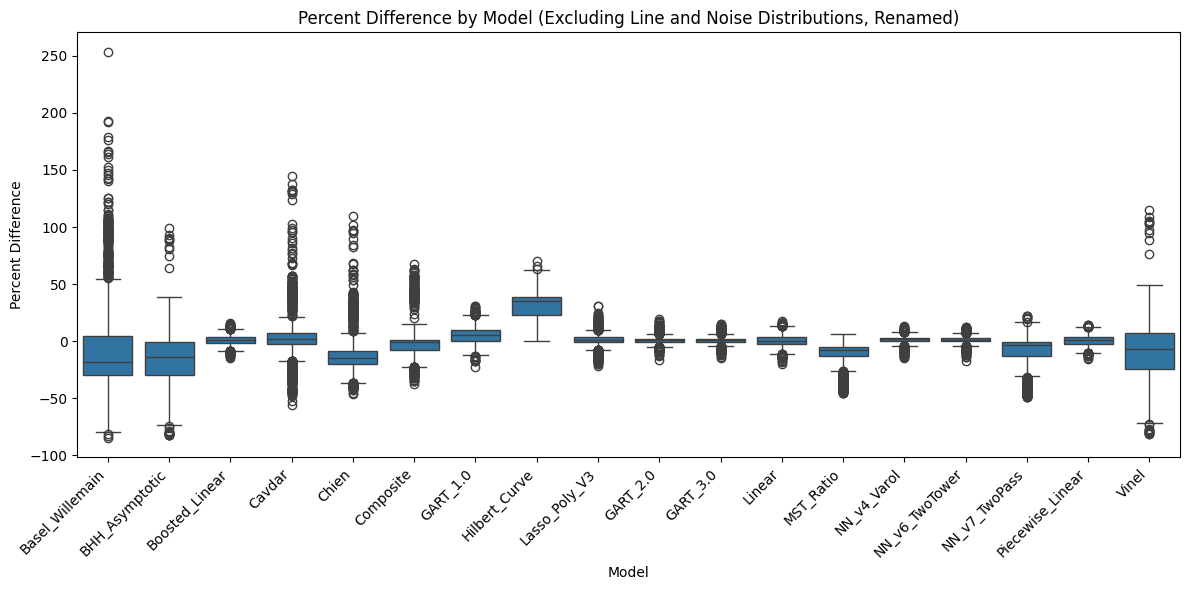
\includegraphics[width=1\linewidth]{2D_noiseless.png}
    \caption{Enter Caption}
    \label{fig:placeholder}
\end{figure}

\begin{table}[H]
    \centering
    \caption{2D Mean and Standard Deviation of Percent Difference (Filtered Data)}
    \label{tab:2d_filtered}
    \begin{tabular}{lS[table-format=3.4]S[table-format=3.4]}
        \toprule
        \textbf{Model} & {\textbf{Mean}} & {\textbf{Std}} \\
        \midrule
        NN\_v4\_Varol & 1.4514 & 3.1251 \\
        GART 2.0 & 1.0840 & 3.4464 \\
        NN\_v6\_TwoTower & 1.2923 & 3.5402 \\
        \textbf{GART 3.0} & \textbf{1.274} & \textbf{3.715} \\
        Boosted\_Linear & 1.0140 & 3.9813 \\
        Piecewise\_Linear & 0.5381 & 4.3806 \\
        Lasso\_Poly\_V3 & 1.2302 & 5.1016 \\
        Linear & 0.7748 & 5.1573 \\
        GART 1.0 & 5.4385 & 6.9303 \\
        MST\_Ratio & -10.2210 & 9.6012 \\
        NN\_v7\_TwoPass & -7.4955 & 11.7379 \\
        Hilbert\_Curve & 30.3485 & 12.6892 \\
        Composite & -1.2836 & 14.4580 \\
        Chien & -12.3880 & 18.2523 \\
        Cavdar & 2.9829 & 19.4726 \\
        BHH\_Asymptotic & -16.9662 & 22.7276 \\
        Vinel & -10.4857 & 24.5014 \\
        Basel\_Willemain & -6.4762 & 37.3581 \\
        \bottomrule
    \end{tabular}
\end{table}

\begin{figure}
    \centering
    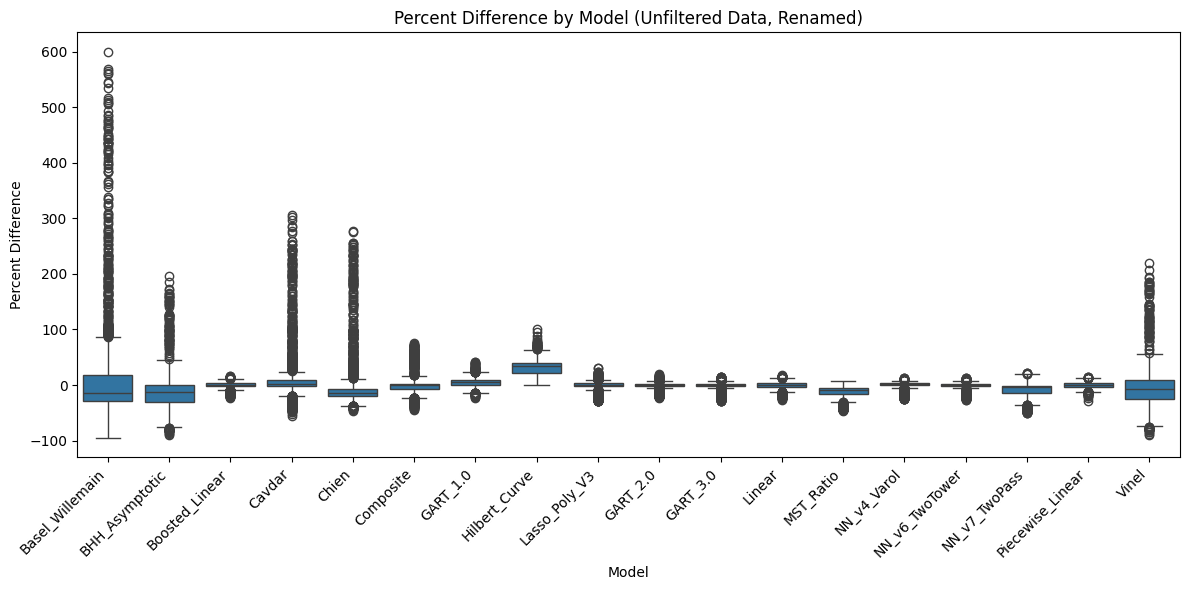
\includegraphics[width=1\linewidth]{2D_all.png}
    \caption{Enter Caption}
    \label{fig:placeholder}
\end{figure}

\begin{table}[H]
    \centering
    \caption{2D Mean and Standard Deviation of Percent Difference (Unfiltered Data)}
    \label{tab:2d_unfiltered}
    \begin{tabular}{lS[table-format=3.4]S[table-format=3.4]}
        \toprule
        \textbf{Model} & {\textbf{Mean}} & {\textbf{Std}} \\
        \midrule
        Piecewise\_Linear & -0.0822 & 5.0296 \\
        GART 2.0 & 0.0783 & 5.1045 \\
        Boosted\_Linear & 0.2630 & 5.2203 \\
        NN\_v6\_TwoTower & 0.2172 & 5.3140 \\
        NN\_v4\_Varol & 0.2748 & 5.3675 \\
        \textbf{GART 3.0} & \textbf{-0.0403} & \textbf{6.1425} \\
        Linear & -0.0773 & 6.4060 \\
        Lasso\_Poly\_V3 & -0.3240 & 7.4993 \\
        GART 1.0 & 5.1812 & 7.9527 \\
        MST\_Ratio & -11.7586 & 11.0557 \\
        NN\_v7\_TwoPass & -9.4262 & 13.5956 \\
        Hilbert\_Curve & 31.0090 & 14.2358 \\
        Composite & 0.4593 & 17.6659 \\
        BHH\_Asymptotic & -13.6626 & 32.0467 \\
        Vinel & -6.9243 & 34.5479 \\
        Cavdar & 11.4205 & 42.0362 \\
        Chien & -3.2799 & 42.5545 \\
        Basel\_Willemain & 13.1064 & 88.3403 \\
        \bottomrule
    \end{tabular}
\end{table}

\subsection{2D Computational Efficiency}

Tables \ref{tab:2d_speedup} through \ref{tab:2d_feature_time} analyze the speed-up factors and execution times for the 2D models.

\begin{table}[H]
    \centering
    \caption{2D Mean and Standard Deviation of Speed-Up Factor}
    \label{tab:2d_speedup}
    \begin{tabular}{lS[table-format=4.2]S[table-format=4.2]}
        \toprule
        \textbf{Model} & {\textbf{Mean}} & {\textbf{Std}} \\
        \midrule
        Chien & 99.40 & 1.35 \\
        Vinel & 97.25 & 4.64 \\
        BHH\_Asymptotic & 96.34 & 5.57 \\
        Cavdar & 95.72 & 6.39 \\
        Hilbert\_Curve & 95.45 & 12.20 \\
        MST\_Ratio & 91.25 & 13.35 \\
        Composite & 87.51 & 19.02 \\
        GART 1.0 & 54.92 & 59.55 \\
        \textbf{GART 3.0} & \textbf{-17.65} & \textbf{156.88} \\
        Lasso\_Poly\_V3 & -47.49 & 191.48 \\
        Linear & -151.01 & 391.59 \\
        GART 2.0 & -178.02 & 318.81 \\
        NN\_v4\_Varol & -209.53 & 354.99 \\
        NN\_v7\_TwoPass & -241.85 & 398.30 \\
        NN\_v6\_TwoTower & -271.49 & 425.78 \\
        Boosted\_Linear & -418.24 & 610.29 \\
        Piecewise\_Linear & -454.47 & 653.35 \\
        Basel\_Willemain & -3160.28 & 4178.66 \\
        \bottomrule
    \end{tabular}
\end{table}

\begin{table}[H]
    \centering
    \caption{2D Average Time (Seconds)}
    \label{tab:2d_avg_time}
    \begin{tabular}{lS[table-format=2.4]S[table-format=2.4]}
        \toprule
        \textbf{Model} & {\textbf{Mean (s)}} & {\textbf{Std (s)}} \\
        \midrule
        Chien & 0.0036 & 0.0058 \\
        Vinel & 0.0064 & 0.0065 \\
        BHH\_Asymptotic & 0.0082 & 0.0062 \\
        Cavdar & 0.0124 & 0.0098 \\
        Hilbert\_Curve & 0.0336 & 0.0486 \\
        MST\_Ratio & 0.0754 & 0.0957 \\
        Composite & 0.0928 & 0.1081 \\
        GART 1.0 & 0.1635 & 0.1292 \\
        \textbf{GART 3.0} & \textbf{0.3343} & \textbf{0.2028} \\
        Lasso\_Poly\_V3 & 0.4264 & 0.2448 \\
        Linear & 0.9986 & 0.7445 \\
        GART 2.0 & 1.1624 & 0.8858 \\
        NN\_v4\_Varol & 1.2374 & 0.8901 \\
        NN\_v7\_TwoPass & 1.3296 & 0.8922 \\
        NN\_v6\_TwoTower & 1.4308 & 0.9665 \\
        Boosted\_Linear & 1.7392 & 1.0714 \\
        Piecewise\_Linear & 1.8806 & 1.1948 \\
        Basel\_Willemain & 11.2048 & 8.5692 \\
        \bottomrule
    \end{tabular}
\end{table}

\begin{table}[H]
    \centering
    \caption{2D Average Inference Time (Seconds)}
    \label{tab:2d_inf_time}
    \begin{tabular}{lS[table-format=1.4]S[table-format=1.4]}
        \toprule
        \textbf{Model} & {\textbf{Mean (s)}} & {\textbf{Std (s)}} \\
        \midrule
        Linear & 0.0053 & 0.0031 \\
        GART 2.0 & 0.0209 & 0.0103 \\
        GART 1.0 & 0.0305 & 0.0159 \\
        Lasso\_Poly\_V3 & 0.0451 & 0.0301 \\
        \textbf{GART 3.0} & \textbf{0.0451} & \textbf{0.0378} \\
        NN\_v4\_Varol & 0.0506 & 0.0231 \\
        NN\_v7\_TwoPass & 0.0617 & 0.0338 \\
        Piecewise\_Linear & 0.0789 & 0.0498 \\
        Boosted\_Linear & 0.0793 & 0.0507 \\
        NN\_v6\_TwoTower & 0.0814 & 0.0368 \\
        \bottomrule
    \end{tabular}
\end{table}

\begin{table}[H]
    \centering
    \caption{2D Average Feature Time (Seconds, Excluding 0 values)}
    \label{tab:2d_feature_time}
    \begin{tabular}{lS[table-format=1.4]S[table-format=1.4]}
        \toprule
        \textbf{Model} & {\textbf{Mean (s)}} & {\textbf{Std (s)}} \\
        \midrule
        GART 1.0 & 0.1330 & 0.1252 \\
        \textbf{GART 3.0} & \textbf{0.2892} & \textbf{0.2039} \\
        Lasso\_Poly\_V3 & 0.3813 & 0.2406 \\
        Linear & 0.9933 & 0.7445 \\
        GART 2.0 & 1.1414 & 0.8851 \\
        NN\_v4\_Varol & 1.1869 & 0.8903 \\
        NN\_v7\_TwoPass & 1.2678 & 0.8928 \\
        NN\_v6\_TwoTower & 1.3494 & 0.9682 \\
        Boosted\_Linear & 1.6599 & 1.0724 \\
        Piecewise\_Linear & 1.8016 & 1.1974 \\
        \bottomrule
    \end{tabular}
\end{table}

\subsection{2D Statistical Significance Tests}

\begin{table}[H]
    \centering
    \caption{Shapiro-Wilk Test P-values for 2D 'percent\_diff' by Model}
    \label{tab:shapiro}
    \begin{tabular}{lS[table-format=1.2e-2]S[table-format=1.2e-2]}
        \toprule
        \textbf{Model} & {\textbf{Unfiltered p-value}} & {\textbf{Filtered p-value}} \\
        \midrule
        Basel\_Willemain & 2.89e-61 & 4.54e-43 \\
        BHH\_Asymptotic & 2.99e-45 & 9.26e-29 \\
        Boosted\_Linear & 7.53e-35 & 1.38e-12 \\
        Cavdar & 8.77e-61 & 6.25e-45 \\
        Chien & 8.26e-62 & 3.45e-44 \\
        Composite & 1.22e-47 & 7.94e-47 \\
        GART 1.0 & 8.61e-22 & 3.44e-19 \\
        Hilbert\_Curve & 1.35e-30 & 2.68e-34 \\
        Lasso\_Poly\_V3 & 2.45e-43 & 3.55e-33 \\
        GART 2.0 & 1.30e-43 & 6.05e-32 \\
        \textbf{GART 3.0} & \textbf{1.22e-48} & \textbf{3.21e-34} \\
        Linear & 4.11e-28 & 3.59e-11 \\
        MST\_Ratio & 4.74e-41 & 2.38e-39 \\
        NN\_v4\_Varol & 7.83e-50 & 2.84e-25 \\
        NN\_v6\_TwoTower & 7.78e-44 & 1.98e-28 \\
        NN\_v7\_TwoPass & 6.29e-40 & 1.37e-37 \\
        Piecewise\_Linear & 4.87e-20 & 4.45e-09 \\
        Vinel & 2.99e-45 & 9.26e-29 \\
        \bottomrule
    \end{tabular}
\end{table}

\begin{table}[H]
    \centering
    \caption{Levene's Test P-values for 2D 'percent\_diff' variance}
    \label{tab:levene}
    \begin{tabular}{lS[table-format=1.2e-2]}
        \toprule
        \textbf{Model} & {\textbf{Levene p-value}} \\
        \midrule
        Basel\_Willemain & 1.48e-25 \\
        BHH\_Asymptotic & 2.05e-10 \\
        Boosted\_Linear & 4.28e-11 \\
        Cavdar & 3.71e-21 \\
        Chien & 5.97e-23 \\
        Composite & 6.60e-07 \\
        GART 1.0 & 8.28e-06 \\
        Hilbert\_Curve & 4.05e-04 \\
        Lasso\_Poly\_V3 & 1.44e-17 \\
        GART 2.0 & 1.10e-15 \\
        \textbf{GART 3.0} & \textbf{1.23e-19} \\
        Linear & 2.20e-09 \\
        MST\_Ratio & 2.05e-07 \\
        NN\_v4\_Varol & 7.66e-23 \\
        NN\_v6\_TwoTower & 2.73e-17 \\
        NN\_v7\_TwoPass & 5.39e-08 \\
        Piecewise\_Linear & 1.37e-06 \\
        Vinel & 2.05e-10 \\
        \bottomrule
    \end{tabular}
\end{table}

\clearpage
\section{N-Dimensional Data Analysis}

The following data pertains to N-Dimensional data. \textbf{GART 3.0} demonstrates superior accuracy with significantly reduced feature computation time compared to prior versions.

\subsection{N-Dimensional Accuracy}

\begin{figure}
    \centering
    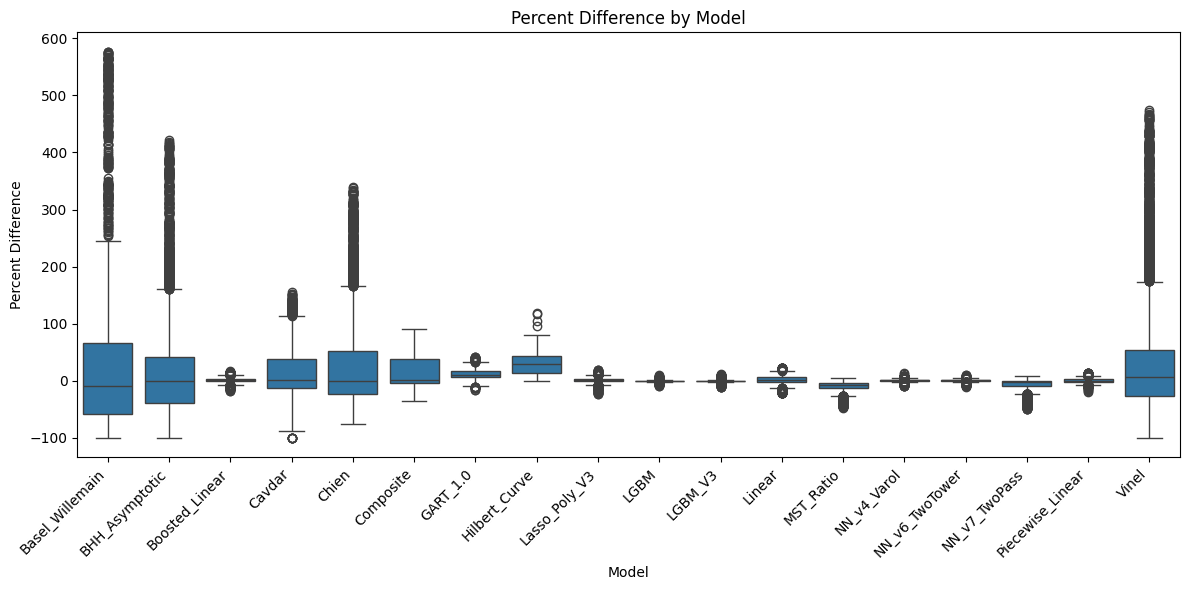
\includegraphics[width=1\linewidth]{ND_all.png}
    \caption{Enter Caption}
    \label{fig:placeholder}
\end{figure}

\begin{table}[H]
    \centering
    \caption{N-Dimensional Mean and Standard Deviation of Percent Difference (Unfiltered Data)}
    \label{tab:ndim_accuracy}
    \begin{tabular}{lS[table-format=3.4]S[table-format=3.4]}
        \toprule
        \textbf{Model} & {\textbf{Mean}} & {\textbf{Std}} \\
        \midrule
        MST\_Ratio & -9.0939 & 8.4333 \\
        NN\_v7\_TwoPass & -5.9764 & 9.5003 \\
        GART 2.0 & 0.0356 & 1.1092 \\
        \textbf{GART 3.0} & \textbf{0.0439} & \textbf{1.5890} \\
        Piecewise\_Linear & 0.4467 & 3.6286 \\
        NN\_v6\_TwoTower & 0.7443 & 1.6647 \\
        Boosted\_Linear & 1.0961 & 3.8996 \\
        NN\_v4\_Varol & 1.1118 & 1.7743 \\
        Lasso\_Poly\_V3 & 1.2531 & 4.0046 \\
        Linear & 2.3858 & 6.3763 \\
        Cavdar & 8.7870 & 44.0824 \\
        GART 1.0 & 11.4382 & 7.9567 \\
        Composite & 15.7170 & 28.7806 \\
        BHH\_Asymptotic & 24.7947 & 95.9572 \\
        Hilbert\_Curve & 29.1202 & 17.5054 \\
        Basel\_Willemain & 30.6214 & 128.0076 \\
        Chien & 32.0631 & 84.4143 \\
        Vinel & 44.2470 & 119.6357 \\
        \bottomrule
    \end{tabular}
\end{table}

\subsection{N-Dimensional Computational Efficiency}

\begin{table}[H]
    \centering
    \caption{N-Dimensional Mean and Standard Deviation of Speed-Up Factor}
    \label{tab:ndim_speedup}
    \begin{tabular}{lS[table-format=4.2]S[table-format=4.2]}
        \toprule
        \textbf{Model} & {\textbf{Mean}} & {\textbf{Std}} \\
        \midrule
        Chien & 99.47 & 1.61 \\
        Hilbert\_Curve & 98.61 & 5.29 \\
        BHH\_Asymptotic & 98.37 & 5.15 \\
        Cavdar & 97.38 & 5.89 \\
        Vinel & 97.18 & 5.93 \\
        MST\_Ratio & 94.95 & 10.40 \\
        Composite & 93.58 & 15.01 \\
        GART 1.0 & 78.97 & 37.04 \\
        Lasso\_Poly\_V3 & 61.20 & 69.50 \\
        \textbf{GART 3.0} & \textbf{49.36} & \textbf{89.24} \\
        Linear & -9.26 & 215.45 \\
        NN\_v7\_TwoPass & -11.66 & 190.25 \\
        GART 2.0 & -15.57 & 195.23 \\
        NN\_v4\_Varol & -23.13 & 208.94 \\
        NN\_v6\_TwoTower & -33.96 & 226.61 \\
        Piecewise\_Linear & -151.79 & 428.50 \\
        Boosted\_Linear & -152.15 & 428.73 \\
        Basel\_Willemain & -1260.17 & 2402.58 \\
        \bottomrule
    \end{tabular}
\end{table}

\begin{table}[H]
    \centering
    \caption{N-Dimensional Average Time (Seconds)}
    \label{tab:ndim_avg_time}
    \begin{tabular}{lS[table-format=2.4]S[table-format=2.4]}
        \toprule
        \textbf{Model} & {\textbf{Mean (s)}} & {\textbf{Std (s)}} \\
        \midrule
        Chien & 0.0073 & 0.0087 \\
        BHH\_Asymptotic & 0.0096 & 0.0092 \\
        Vinel & 0.0135 & 0.0097 \\
        Cavdar & 0.0167 & 0.0125 \\
        Hilbert\_Curve & 0.0226 & 0.0273 \\
        MST\_Ratio & 0.0871 & 0.0729 \\
        Composite & 0.1042 & 0.0832 \\
        GART 1.0 & 0.1584 & 0.0910 \\
        Lasso\_Poly\_V3 & 0.2403 & 0.1175 \\
        \textbf{GART 3.0} & \textbf{0.2902} & \textbf{0.1262} \\
        NN\_v7\_TwoPass & 1.0827 & 0.6984 \\
        Linear & 1.0958 & 0.7755 \\
        NN\_v4\_Varol & 1.1734 & 0.7923 \\
        GART 2.0 & 1.1927 & 0.8520 \\
        NN\_v6\_TwoTower & 1.2299 & 0.8232 \\
        Boosted\_Linear & 1.9201 & 1.1765 \\
        Piecewise\_Linear & 1.9457 & 1.2146 \\
        Basel\_Willemain & 12.4895 & 9.1979 \\
        \bottomrule
    \end{tabular}
\end{table}

\begin{table}[H]
    \centering
    \caption{N-Dimensional Average Inference Time (Seconds)}
    \label{tab:ndim_inf_time}
    \begin{tabular}{lS[table-format=1.4]S[table-format=1.4]}
        \toprule
        \textbf{Model} & {\textbf{Mean (s)}} & {\textbf{Std (s)}} \\
        \midrule
        Linear & 0.0055 & 0.0030 \\
        Lasso\_Poly\_V3 & 0.0153 & 0.0099 \\
        GART 2.0 & 0.0196 & 0.0074 \\
        \textbf{GART 3.0} & \textbf{0.0200} & \textbf{0.0095} \\
        GART 1.0 & 0.0268 & 0.0111 \\
        NN\_v4\_Varol & 0.0548 & 0.0175 \\
        Piecewise\_Linear & 0.0645 & 0.0313 \\
        Boosted\_Linear & 0.0732 & 0.0345 \\
        NN\_v7\_TwoPass & 0.0732 & 0.0232 \\
        NN\_v6\_TwoTower & 0.0923 & 0.0236 \\
        \bottomrule
    \end{tabular}
\end{table}

\begin{table}[H]
    \centering
    \caption{N-Dimensional Average Feature Time (Seconds)}
    \label{tab:ndim_feature_time}
    \begin{tabular}{lS[table-format=1.4]S[table-format=1.4]}
        \toprule
        \textbf{Model} & {\textbf{Mean (s)}} & {\textbf{Std (s)}} \\
        \midrule
        GART 1.0 & 0.1316 & 0.0905 \\
        Lasso\_Poly\_V3 & 0.2250 & 0.1172 \\
        \textbf{GART 3.0} & \textbf{0.2702} & \textbf{0.1260} \\
        NN\_v7\_TwoPass & 1.0095 & 0.6976 \\
        Linear & 1.0902 & 0.7753 \\
        NN\_v4\_Varol & 1.1186 & 0.7918 \\
        NN\_v6\_TwoTower & 1.1376 & 0.8220 \\
        GART 2.0 & 1.1731 & 0.8519 \\
        Boosted\_Linear & 1.8469 & 1.1807 \\
        Piecewise\_Linear & 1.8812 & 1.2188 \\
        \bottomrule
    \end{tabular}
\end{table}

\end{document}